\documentclass[11pt]{article}
\usepackage{amsmath}
\usepackage{graphicx}
\usepackage{hyperref}
\usepackage[utf8]{inputenc}
\usepackage[spanish]{babel}
\usepackage[margin=2cm]{geometry}
\usepackage{amsfonts}
\usepackage{listings}
\usepackage[T1]{fontenc}
\usepackage{float}

\title{Práctica Mineria de Flujo de Datos.}
\author{Néstor Rodríguez Vico. DNI: 75573052C - \href{mailto:nrv23@correo.ugr.es}{nrv23@correo.ugr.es}}
\date{\today}


\lstdefinestyle{bash_style}{
	language=bash,
	frame=single,
	xleftmargin=.25in,
	upquote = true,
	basicstyle=\scriptsize,
	breakatwhitespace=false,         
	breaklines=true,                 
	captionpos=b,                    
	keepspaces=true,                 
	numbers=left,                    
	numbersep=5pt,                  
	showspaces=false,                
	showstringspaces=false,
	showtabs=false,                  
	tabsize=2
}

\lstset{style=bash_style}

\begin{document}
\maketitle

\setlength{\belowdisplayskip}{5pt} 
\setlength{\belowdisplayshortskip}{5pt}
\setlength{\abovedisplayskip}{5pt} 
\setlength{\abovedisplayshortskip}{5pt}

\section{Parte teórica.}

\subsection{Preguntas tipo test.}

\textbf{Responda a las 12 preguntas tipo test del anexo. Cada respuesta incorrecta restará un tercio (si hay cuatro opciones) o una unidad (si tiene dos opciones) del valor de cada pregunta (un doceavo).}

\begin{enumerate}
	\item \textit{El aprendizaje incremental es últil cuando...} d) se quiere ganar eficiencia.
	\item \textit{La minería de flujo de datos se considera cuando...} a) el problema genera datos continuamente.
	\item \textit{La cota de Hoeffding sirve para saber...} b) cuando hay suficientes datos para una estimación fiable.
	\item \textit{¿Que características de clusters mantiene el algoritmo BIRCH?} d) Suma linea, suma cuadrática y número de objetos.
	\item \textit{¿El algoritmo Stram maneja concept drift?} b) No.
	\item \textit{¿Qué es concept drift?} d) Cambios en la dinámica del problema.
	\item \textit{¿Cómo gestion CVFDT el concept drift?} d) Mantiene árboles alternativos.
	\item \textit{¿Por qué es útil el ensemble learning en concept drift?} c) Porque mantienen muchos modelos simultáneamente.
	\item \textit{¿Cuál es más eficiente entre DDM y ADWIN?}: c) ADAWIN es más eficiente.
	\item \textit{¿Por qué es controvertida la clasificación en flujo de datos?} a) Porque se requiere al oráculo por siempre.
	\item \textit{¿Cómo gestiona ClueStream el concept drift?}
	\item \textit{¿Por qué es complejo generar reglas de asociación en flujo de datos?}
\end{enumerate}

\newpage
\subsection{Pregunta 1.}

\textbf{Explique el problema de clasificación, los clasificadores utilizados en los experimentos de la sección 2, y en qué consisten los diferentes modos de evaluación/validación en flujos de datos. Desarrolle con suficiente detalle este apartado.} \\

En el problema de clasificación en flujo de datos no se disponen de los datos previamente. En estos problemas, los datos van llegando conforme pasa el tiempo. Debido a la cantidad de datos producidos, lo que se suele hacer es procesar el dato y, seguídamente, descartarlo. Al igual que en propblemas de clasificación estándar, los algoritmos usado en clasificación en flujo de datos deben ser capaces de maximizar la precisión. De forma adicional, estos algoritmos deben ser capaces de detectar y reaccionar ante los cambios de concepto que se pueden producir. \\

Los algoritmos usados en la parte de prácticas son: 

\begin{itemize}
	\item \textit{HoeffdingTree:} Se trata de un algoritmo que permite construir un árbol incremental a partir de un flujo de datos, asumiendo que  no se producen cambios de convepto en el flujo de datos. La principal característica de este algoritmo es que hace uso de un valor denominado \textit{cota de Hoeffding}, la cual representa el número de instancias necesarias para calcular los datos estadísticos de un flujo de datos de forma precisa. Esta cota es usada para decidir cuando vamos a dividir un nodo. 
	\item \textit{HoeffdingAdaptiveTree:} La diferencia de \textit{HoeffdingAdaptiveTree} con \textit{HoeffdingTree} es que usa \textit{ADWIN} para analizar el rendimiento de las ramas del árbol, lo cual permite reemplazarlas por nuevas si su rendimiento decrece.
\end{itemize}

Los modelos de evaluación empleados son:

\begin{itemize}
	\item \textit{EvaluateModel:} Se produce una evluación estática del modelo.
	\item \textit{InterleavedTest-Then-Train:} cuando llega un dato nuevo se usa para evaluar el modelo y, a continuación, se le da al modelo para que lo aprenda.
	\item \textit{Prequential:} técnica que permite usar una ventana deslizante para olvidar instancias antiguas.
\end{itemize}

\subsection{Pregunta 2.}

\textbf{Explique en qué consiste el problema de concept drift y qué técnicas conoce para resolverlo en clasificación. Desarrolle con suficiente detalle este apartado.} \\

Una de las principales dificultades que se aborda en flujo de datos es el desvío de concepto o concept drift, esto es, un cambio en la dinámica de los datos. Este cambio puede ser de tres tipos:

\begin{itemize}
	\item Repentino: se produce un cambio de forma rápida.
	\item Incremental: el cambio en la dinámica del flujo de datos se produce lentamente.
	\item Gradual: el cambio de produce de forma lenta y, por lo tanto, hay un periodo de tiempo en el que ambas dinámicas (la antigua y la nueva) coexisten en el flujo de datos.
	\item Recurrente: el cambio en la dinámica se produce varias veces a lo largo del flujo de datos.
\end{itemize}

Las técnicas usadas para abordar el \textit{Concept Drift} pueden dividirse en los siguientes enfoques:

\begin{itemize}
	\item \textit{Aprendizaje online:} Aquí encontramos los clasificadores que se actualizan con cada nueva instancia. No todos los clasificadores pueden actuar como aprendizaje online, tienen que cumplir una serie de requisitos básicos. Primero: cada objeto debe procesarse solo una vez durante el entrenamiento. Segundo: el sistema debe consumir una memoria y procesamiento limitados con independencia de la cantidad de datos procesada. Tercero: el aprendizaje se puede pausar en cualquier momento y su precisión no debería ser peor que la de un clasificador entrenado offline sobre los datos vistos hasta el momento.
	\item \textit{Soluciones basadas en instancias (ventana):} Aquí encontramos los algoritmos que incorporan mecanismos para olvidar datos antiguos. Se basan en asumir que los datos llegados recientemente son más relevantes porque contienen características del contexto actual y su relevancia disminuye con el paso del tiempo. Por tanto, ajustar el rango de datos a aquellos que han llegado más recientemente puede ayudar a formar un conjunto de datos que representa al contexto actual.
	\item \textit{Aprendizaje de múltiples modelos (ensemble):} Entre los enfoques ensemble para flujo de datos más populares, podemos destacar:
	\textit{Streaming Ensemble Algorithm (SEA)} y \textit{Accuracy Weighted Ensemble (AWE)}. Ambos algoritmos mantienen un número fijo de clasificadores. Los datos que van llegando se recogen en fragmentos que se usan para entrenar nuevos clasificadores. Los clasificadores se evalúan según su precisión y el peor es reemplazado por uno nuevo si este último es más preciso. \textit{SEA} usa voto por mayoría, mientras que \textit{AWE} usa un voto ponderado.
	\item \textit{Algoritmos de detección del desvío:} En lugar de dotar de adaptabilidad al proceso de aprendizaje, otra alternativa es detectar cuándo se produce el \textit{Concept Drift} y actuar para paliar sus efectos (por ejemplo, reseteando total o parcialmente el conocimiento adquirido por el algoritmo). El objetivo de cualquier detector de \textit{Concept Drift} es reconocer los cambios en flujos de datos no estacionarios de manera precisa y oportuna. El algoritmo explicado en clase de este enfoque es \textit{DDM (Drift Detection Method)}. \textit{DDM} detecta el desvío de concepto en función de la precisión del clasificador o mediante un análisis de distribución de la clase. Para ello, almacena datos estadísticos de dos ventanas de tiempo. La primera de ellas contiene información de los errores obtenidas durante todo el proceso. La segunda contiene los datos desde el inicio hasta que el error empieza a incrementar considerablemente, es decir, cuando se empieza a producir el cambio de convepto. \textit{DDM} se comporta bien si el cambio de concepto es bruscos, pero no se comporate bien cuando el cambio es lento. Otro algoritmo es \textit{ADAWIN (ADaptive sliding WINdow)}. Dada la ventana $W$, si existen dos subventanas $W_0$ y $W_1$ suficientemente grandes y con medias suficientemente distintas, podemos concluir que los valores esperados son diferentes y se puede eliminar la parte antigua de $W$. Finalmente, otro algoritmo que podemose usar es \textit{HSP}. \textit{HSP} basa la deteccioón exclusivamente en las muestras, sin necesidad de monitorizar al algoritmo, con las siguientes ventajas:
	\begin{itemize}
		\item Complejidad de tiempo y espacio O(nm) -siendo \textit{n} el número de características y \textit{m} el número de clases- para procesar cada muestra: es extremadamente eficiente.
		\item Implementación e integración ágil, lo que facilita la creación de prototipos y el análisis exploratorio de nuevos problemas de flujo de datos. Su diseño es simple, por lo que es fácil de entender su comportamiento y depurar el proceso.
		\item La verdadera detección de \textit{Concept Drift}, incluso cuando los algoritmos eficaces no se degradan significativamente, puede mejorar el proceso de predicción y obtener una mayor comprensión sobre la naturaleza del problema.
		\item En último término, \textit{HSP} es compatible con el uso de detectores de \textit{Concept Drift} tradicionales basados en el rendimiento del algoritmo, por lo que se pueden complementar para corroborar detecciones o adaptarse dinámicamente a las características del problema.
	\end{itemize}
\end{itemize}

\section{Parte práctica.}

Para ejecutar los experimentos de esta sección se ha usado el mismo script que se ha usado en el trabajo guiado:

\begin{lstlisting}[language=bash]
for i in $(seq 5)
do
	java -cp moa.jar -javaagent:sizeofag-1.0.0.jar moa.DoTask "..." > "$i.txt"
done
\end{lstlisting}

Sólo debemos cambiar los tres puntos de la línea 3 por la orden que queramos ejecutar. Una vez tenemos los resultados de las 5 ejecuciones, podemos aplicar los tests estadísticos. Para ello, he usado el siguiente código en R:

\begin{lstlisting}[language=R]
read.data <- function(folder, col) {
	# Listamos los ficheros
	ficheros <- list.files(path = folder, full.names=TRUE)
	# Leemos los conjuntos de datos
	data <- lapply(ficheros, read.csv)
	# Tal y como dice la transparencia 19, nos quedamos el 
	# ultimo valor de la columna deseada.
	sapply(data, function(x) x[nrow(x), col])
}

accuracy.standard <- read.data(folder = "...", col = 5)
kappa.standard <- read.data(folder = "...", col = 6)
accuracy.adaptative <- read.data(folder = "...", col = 5)
kappa.adaptative <- read.data(folder = "...", col = 6)
\end{lstlisting}

Este código simplemente lee todos los ficheros almacenados en un directorio (que son los obtenido con el script anterior) y selecciona el último valor de la columna indicada, para así obtener la tasa de aciertos y el valor \textit{Kappa} para cada ejecución con una semilla distinta. Esos valores los almacena en un vector que será usado posteriormente.

\subsection{Entrenamiento offline (estacionario) y evaluación posterior.}

\subsubsection{Ejercicio 1.}

\textbf{Entrenar un clasificador HoeffdingTree offline (estacionario, aprender modelo únicamente), sobre un total de 1.000.000 de instancias procedentes de un flujo obtenido por el generador WaveFormGenerator con semilla aleatoria igual a 2. Evaluar posteriormente (sólo evaluación) con 1.000.000 de instancias generadas por el mismo tipo de generador, con semilla aleatoria igual a 4. Repita el proceso varias veces con la misma semilla en evaluación y diferentes semillas en entrenamiento, para crear una población de resultados. Anotar como resultados los valores de porcentajes de aciertos en la clasificación y estadístico Kappa.} \\

Para resolver este problema se ha usado la siguiente orden:

\begin{lstlisting}[language=bash]
EvaluateModel -m
	(LearnModel 
		-l trees.HoeffdingTree 
		-s (generators.WaveformGenerator -i 2) 
		-m 1000000
	) -s (generators.WaveformGenerator -i 4) -i 1000000
\end{lstlisting}

En la línea tres difinimos el modelo que vamos a aprender. En la línea cuatro indicamos como se van a generar los datos, en este caso usando el generador \textit{WaveFormGenerator} con semilla \textit{2}. En la línea cinco indicamos el número de instancias a generar. Finalmente, en la línea seis evaluamos el modelo con 100000 instancias generador por el generado \textit{WaveFormGenerator} con semilla \textit{4}. Para automatizar la prueba de varias semillas voy a usar el script comentado al principio de la parte práctica y modificar el comando de \textit{MOA} para que la semilla de entrenamiento sea distinta. Los resultados obtenidos son los siguientes:

\begin{table}[H]
	\centering
	\begin{tabular}{rcc}
		\textbf{Semilla} & \textbf{\% Acierto} & \textbf{Kappa} \\ \hline
		1 & 84.509 & 76.765 \\
		2 & 84.512 & 76.770 \\
		3 & 84.590 & 76.887 \\
		4 & 84.666 & 77.001 \\
		5 & 84.481 & 76.723
	\end{tabular}
\end{table}

\subsubsection{Ejercicio 2.}

\textbf{Repetir el paso anterior, sustituyendo el clasificador por HoeffdingTree adaptativo.} \\

Para resolver este problema se ha usado la siguiente orden:

\begin{lstlisting}[language=bash]
EvaluateModel -m
	(LearnModel 
		-l trees.HoeffdingAdaptiveTree 
		-s (generators.WaveformGenerator -i 2) 
		-m 1000000
	) -s (generators.WaveformGenerator -i 4) -i 1000000
\end{lstlisting}

El código es el mismo, sólo tenemos que cambiar el modelo que vamos a aprender en la línea 3. Los resultados obtenidos son los siguientes:

\begin{table}[H]
	\centering
	\begin{tabular}{rcc}
		\textbf{Semilla} & \textbf{\% Acierto} & \textbf{Kappa} \\ \hline
		1 & 84.521 & 76.783 \\
		2 & 84.474 & 76.712 \\
		3 & 84.416 & 76.625 \\
		4 & 84.465 & 76.699 \\
		5 & 84.262 & 76.395
	\end{tabular}
\end{table}

\subsubsection{Ejercicio 3.}

\textbf{Responda a la pregunta: ¿Cree que algún clasificador es significativamente mejor que el otro en este tipo de problemas? Razone su respuesta.} \\

Para responder a esta pergunta podríamos usar un test de \textit{Student}, al igual que hemos hecho en el trabajo guiado. Para ello, primero debemos comprobar la normalidad de los datos. Este proceso se va a hacer con R:

\begin{lstlisting}
accuracy.estandar <- c(84.509, 84.512, 84.590, 84.666, 84.481)
kappa.estandar <- c(76.765, 76.770, 76.887, 77.001, 76.723)

accuracy.adaptative <- c(84.521, 84.474, 84.416, 84.465, 84.262)
kappa.adaptative <- c(76.783, 76.712, 76.625, 76.699, 76.395)

shapiro.test(accuracy.standar)$p.value # 0.3359973
shapiro.test(kappa.standar)$p.value # 0.340034
shapiro.test(accuracy.adaptative)$p.value # 0.2657517
shapiro.test(kappa.adaptative)$p.value # 0.2691799
\end{lstlisting}

Cómo podemos ver, los datos son normales, así que podemos aplicar un test de \textit{Student}:

\begin{lstlisting}
t.test(accuracy.standar, accuracy.adaptative)$p.value # 0.06014706
t.test(kappa.standar, kappa.adaptative)$p.value # 0.05956797
\end{lstlisting}

Los test no pasan, ya que el p-valor obtenido es mayor que 0.05, lo cual nos indica que no hay diferencia entre los algoritmos.

\subsection{Entrenamiento online.}

\subsubsection{Ejercicio 1.}

\textbf{Entrenar un clasificador HoeffdingTree online, mediante el método Interleaved Test-Then-Train, sobre un total de 1.000.000 de instancias procedentes de un flujo obtenido por el generador WaveFormGenerator con semilla aleatoria igual a 2, con una frecuencia de muestreo igual a 10.000. Pruebe con otras semillas aleatorias para crear una población de resultados. Anotar los valores de porcentajes de aciertos en la clasificación y estadístico Kappa.} \\

Para resolver este problema se ha usado la siguiente orden:

\begin{lstlisting}[language=bash]
EvaluateInterleavedTestThenTrain -l trees.HoeffdingTree
	-s (generators.WaveformGenerator -i 2)
	-i 1000000
	-f 10000
\end{lstlisting}

La idea de este comando es bastante similar al usado en el ejercicio anterior. Primero definimos el método a usar y el modelo en la línea uno, a continuación generamos los datos usando un generado \textit{WaveformGenerator} como podemos ver en la línea dos. Finalmente, definimos los datos usado por el experimento en la línea tres y cuatro. Los resultados obtenidos son los siguientes:

\begin{table}[H]
	\centering
	\begin{tabular}{rcc}
		\textbf{Semilla} & \textbf{\% Acierto} & \textbf{Kappa} \\ \hline
		1 & 83.8903 & 75.836 \\
		2 & 83.7851 & 75.677 \\
		3 & 83.8876 & 75.829 \\
		4 & 84.0451 & 76.069 \\
		5 & 83.8402 & 75.759
	\end{tabular}
\end{table}

\subsubsection{Ejercicio 2.}

\textbf{Repetir el paso anterior, sustituyendo el clasificador por HoeffdingTree adaptativo.} \\

Para resolver este problema se ha usado la siguiente orden:

\begin{lstlisting}[language=bash]
EvaluateInterleavedTestThenTrain -l trees.HoeffdingAdaptativeTree
	-s (generators.WaveformGenerator -i 2)
	-i 1000000
	-f 10000
\end{lstlisting}

El código es el mismo, sólo tenemos que cambiar el modelo que vamos a aprender en la línea uno. Los resultados obtenidos son los siguientes:

\begin{table}[H]
	\centering
	\begin{tabular}{rcc}
		\textbf{Semilla} & \textbf{Kappa} & \textbf{\% Acierto} \\ \hline
		1 & 75.707 & 83.8042 \\
		2 & 75.596 & 83.7313 \\
		3 & 75.679 & 83.7875 \\
		4 & 75.696 & 83.7961 \\
		5 & 75.571 & 83.7144
	\end{tabular}
\end{table}

\subsubsection{Ejercicio 3.}

\textbf{Responda a la pregunta: ¿Cree que alguún clasificador es mejor que el otro en este tipo de problemas? Razone su respuesta.} \\

Para responder a esta pergunta podríamos usar un test de \textit{Student}, al igual que hemos hecho en el trabajo guiado. Para ello, primero debemos comprobar la normalidad de los datos. Este proceso se va a hacer con R:

\begin{lstlisting}
shapiro.test(accuracy.standard)$p.value # 0.4709823
shapiro.test(kappa.standard)$p.value # 0.4709826
shapiro.test(accuracy.adaptative)$p.value # 0.1879361
shapiro.test(kappa.adaptative)$p.value # 0.2112991

tseries::jarque.bera.test(accuracy.standard)$p.value # 0.7643144
tseries::jarque.bera.test(kappa.standard)$p.value # 0.759523
tseries::jarque.bera.test(accuracy.adaptative)$p.value # 0.6988181
tseries::jarque.bera.test(kappa.adaptative)$p.value # 0.7029419
\end{lstlisting}

Cómo podemos ver, los datos son normales, así que podemos aplicar un test de \textit{Student}:

\begin{lstlisting}
t.test(accuracy.standard, accuracy.adaptative)$p.value # 0.04417184
t.test(kappa.standard, kappa.adaptative)$p.value # 0.04499021
\end{lstlisting}

Los test si pasan, ya que el p-valor obtenido es menor que 0.05, lo cual nos indica que hay diferencia entre los algoritmos. Para decidir cual es el mejor, simplemente calculamos la media de acierto:

\begin{lstlisting}
mean(accuracy.standard) # 83.88966
mean(accuracy.adaptative) # 83.7667
\end{lstlisting}

En este caso, usar \textit{HoeffdingTree} proporciona unos mejores resultados que \textit{HoeffdingAdaptiveTree}.

\subsection{Entrenamiento online en datos con concept drift.}

\subsubsection{Ejercicio 1.}

\textbf{Entrenar un clasificador HoeffdingTree online, mediante el método Interleaved Test-Then-Train, sobre un total de 2.000.000 de instancias muestreadas con una frecuencia de 100.000, sobre datos procedentes de un generador de flujos RandomRBFGeneratorDrift, con semilla aleatorio igual a 1 para generación de modelos y de instancias, generando 2 clases, 7 atributos, 3 centroides en el modelo, drift en todos los centroides y velocidad de cambio igual a 0.001. Pruebe con otras semillas aleatorias. Anotar los valores de porcentajes de aciertos en la clasificación y estadístico Kappa. Compruebe la evolución de la curva de aciertos en la GUI de MOA.} \\

Para resolver este problema se ha usado la siguiente orden:

\begin{lstlisting}[language=bash]
EvaluateInterleavedTestThenTrain -l trees.HoeffdingTree
	-s (generators.RandomRBFGeneratorDrift 
		-r 1 
		-i 1 
		-a 7 
		-n 3
		-k 3 
		-s 0.001 
	) -i 2000000
	-f 100000
\end{lstlisting}

En la lína uno indicamos el modelo a aprender. En la línea se indica el generador de flujos a usar, \textit{RandomRBFGeneratorDrift}. De las líneas tres a ocho indicamos los parámetros de dicho generador de datos. Línea tres: semilla para la generación del modelo. Línea cuatro: semilla para la generación de instancias. Línea cinco: número de atributos a generar. Línea seis: número de centroides a generar. Línea siete: número de centroides con drift. Línea ocho: velocidad de cambio. Finalmente, en la línea nueve indicamos que vamos a generar 2000000 instancias y en la línea diez que la frecuencia de muestreo va a ser 100000. Las semillas se han cambiado tanto para la generación del modelo como para la generación de las instancias. Los resultados obtenidos son los siguientes:

\begin{table}[H]
	\centering
	\begin{tabular}{rcc}
		\textbf{Semilla} & \textbf{\% Acierto} & \textbf{Kappa} \\ \hline
		1 & 77.454 & 54.775 \\
		2 & 83.956 & 29.391 \\
		3 & 73.473 & 43.058 \\
		4 & 73.046 & 44.985 \\
		5 & 72.061 & 43.152
	\end{tabular}
\end{table}

La evolución de la curva de aciertos es la siguiente:

\begin{figure}[H]
	\centering
	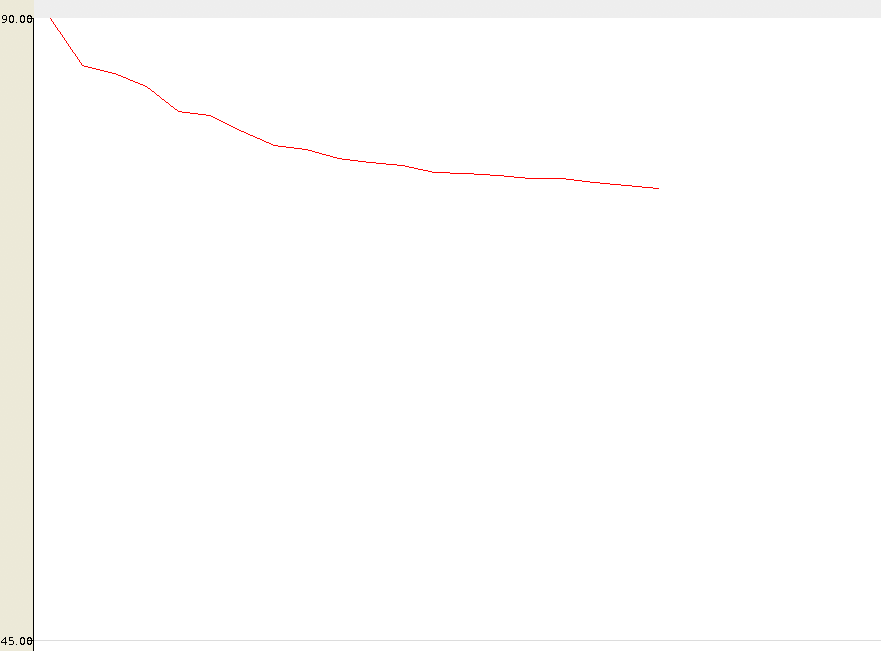
\includegraphics[width=0.5\linewidth]{2_3_1.png}
\end{figure}

Como podemos ver, la curva de aciertos es decreciente, es decir, conforme va pasando el tiempo, el modelo es peor.

\subsubsection{Ejercicio 2.}

\textbf{Repetir el paso anterior, sustituyendo el clasificador por HoeffdingTree adaptativo.} \\

Para resolver este problema se ha usado la siguiente orden:

\begin{lstlisting}[language=bash]
EvaluateInterleavedTestThenTrain -l trees.HoeffdingAdaptiveTree
	-s (generators.RandomRBFGeneratorDrift 
		-r 1 
		-i 1 
		-a 7 
		-n 3
		-k 3 
		-s 0.001 
	) -i 2000000
	-f 100000
\end{lstlisting}

El código es el mismo, sólo tenemos que cambiar el modelo que vamos a aprender en la línea uno. Las semillas se han cambiado tanto para la generación del modelo como para la generación de las instancias. Los resultados obtenidos son los siguientes:

\begin{table}[H]
	\centering
	\begin{tabular}{rcc}
		\textbf{Semilla} & \textbf{\% Acierto} & \textbf{Kappa} \\ \hline
		1 & 96.249 & 92.491 \\
		2 & 92.647 & 73.926 \\
		3 & 96.309 & 92.194 \\
		4 & 95.983 & 91.771 \\
		5 & 90.996 & 81.657
	\end{tabular}
\end{table}

La evolución de la curva de aciertos es la siguiente:

\begin{figure}[H]
	\centering
	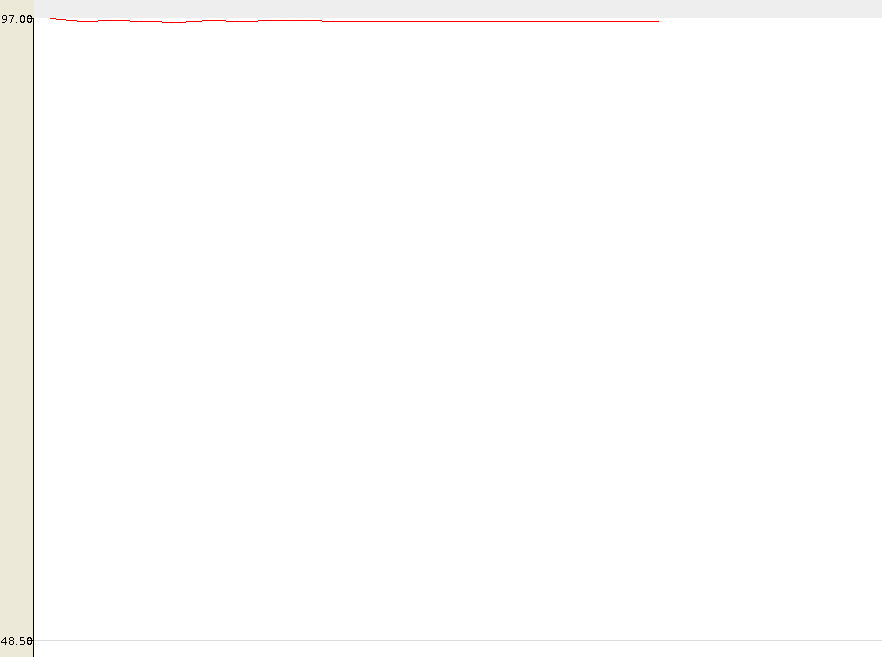
\includegraphics[width=0.5\linewidth]{2_3_2.png}
\end{figure}

Como podemos ver, la curva de aciertos en este caso es más estables, es decir, conforme va pasando el tiempo, el modelo mantiene su calidad, lo cual nos hace pensar que \textit{HoeffdingAdaptiveTree} es mejor que \textit{HoeffdingTree}.

\subsubsection{Ejercicio 3.}

\textbf{Responda a la pregunta: ¿Cree que algún clasificador es mejor que el otro en este tipo de problemas? Razone su respuesta.} \\

Para responder a esta pergunta podríamos usar un test de \textit{Student}, al igual que hemos hecho en el trabajo guiado. Para ello, primero debemos comprobar la normalidad de los datos. Este proceso se va a hacer con R:

\begin{lstlisting}
shapiro.test(accuracy.standard)$p.value # 0.1587713
shapiro.test(kappa.standard)$p.value # 0.5099431
shapiro.test(accuracy.adaptative)$p.value # 0.08033221
shapiro.test(kappa.adaptative)$p.value # 0.07773439

tseries::jarque.bera.test(accuracy.standard)$p.value # 0.6533606
tseries::jarque.bera.test(kappa.standard)$p.value # 0.9239095
tseries::jarque.bera.test(accuracy.adaptative)$p.value # 0.6975661
tseries::jarque.bera.test(kappa.adaptative)$p.value # 0.6996095
\end{lstlisting}

Cómo podemos ver, los datos son normales, así que podemos aplicar un test de \textit{Student}:

\begin{lstlisting}
t.test(accuracy.standard, accuracy.adaptative)$p.value # 0.0003108372
t.test(kappa.standard, kappa.adaptative)$p.value # 5.072058e-05
\end{lstlisting}

Los test si pasan, ya que el p-valor obtenido es menor que 0.05, lo cual nos indica que hay diferencia entre los algoritmos. Para decidir cual es el mejor, simplemente calculamos la media de acierto:

\begin{lstlisting}
mean(accuracy.standard) # 75.99857
mean(accuracy.adaptative) # 94.43709
\end{lstlisting}

En este caso, usar \textit{HoeffdingAdaptiveTree} proporciona unos resultados bastante superiores a \textit{HoeffdingTree}.

\subsection{Entrenamiento online en datos con concept drift, incluyendo mecanismos para olvidar instancias pasadas.}

\subsubsection{Ejercicio 1.}

\textbf{Repita la experimentación del apartado anterior, cambiando el método de evaluación ``Interleaved Test-Then-Train'' por el método de evaluación ``Prequential'', con una ventana deslizante de tamaño 1.000.} \\

Para resolver este problema se ha usado la siguiente orden:

\begin{lstlisting}[language=bash]
EvaluatePrequential -l trees.HoeffdingTree
	-s (generators.RandomRBFGeneratorDrift 
		-r 1 
		-i 1 
		-a 7 
		-n 3
		-k 3 
		-s 0.001 
	) -i 2000000
-f 100000
\end{lstlisting}

El código es el mismo que en el experimento anterior, sólo tenemos que cambiar el método de evaluación en la línea uno. Las semillas se han cambiado tanto para la generación del modelo como para la generación de las instancias. Los resultados obtenidos son los siguientes:

\begin{table}[H]
	\centering
	\begin{tabular}{rcc}
		\textbf{Semilla} & \textbf{\% Acierto} & \textbf{Kappa} \\ \hline
		1 & 76.6 & 52.558 \\
		2 & 86.5 & 39.825 \\
		3 & 52.9 & -0.106 \\
		4 & 65.3 & 29.603 \\
		5 & 63.3 & 25.284
	\end{tabular}
\end{table}

A continuación se ha pasado a usar un modelo \textit{HoeffdingAdaptiveTree}. Para ello se ha usado la siguiente orden:

\begin{lstlisting}[language=bash]
EvaluatePrequential -l trees.HoeffdingAdaptiveTree
	-s (generators.RandomRBFGeneratorDrift 
		-r 1 
		-i 1 
		-a 7 
		-n 3
		-k 3 
		-s 0.001 
	) -i 2000000
-f 100000
\end{lstlisting}

El código es el mismo, sólo tenemos que cambiar el método de evaluación en la línea uno. Las semillas se han cambiado tanto para la generación del modelo como para la generación de las instancias. Los resultados obtenidos son los siguientes:

\begin{table}[H]
	\centering
	\begin{tabular}{rcc}
		\textbf{Semilla} & \textbf{\% Acierto} & \textbf{Kappa} \\ \hline
		1 & 96.6 & 93.190 \\
		2 & 95.3 & 82.198 \\
		3 & 98.0 & 95.755 \\
		4 & 96.3 & 92.468 \\
		5 & 91.9 & 83.400
	\end{tabular}
\end{table}

Las curvas de acierto son las siguientes:

\begin{table}[H]
	\centering
	\begin{tabular}{cc}
	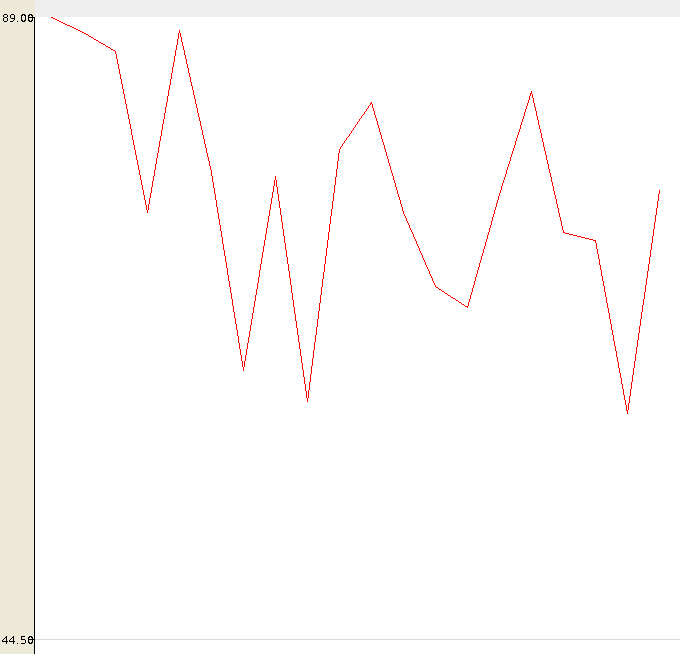
\includegraphics[width=0.4\linewidth]{2_4_1.png} & 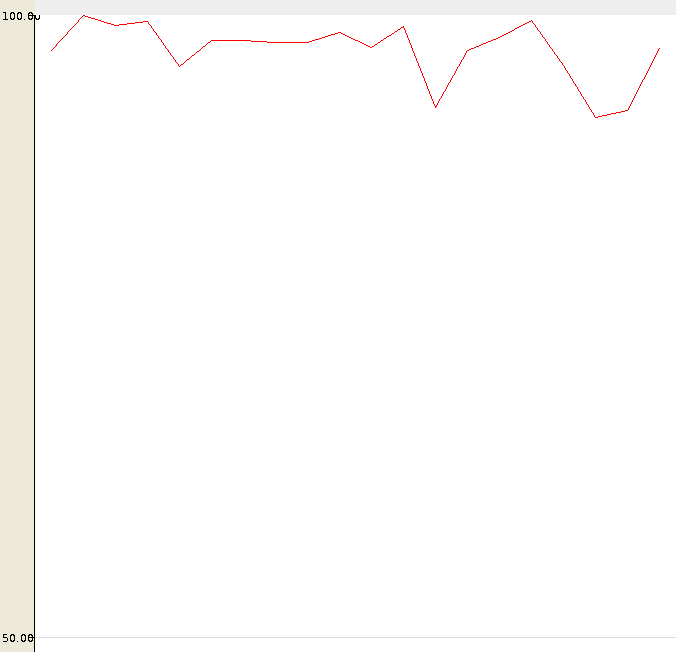
\includegraphics[width=0.4\linewidth]{2_4_2.png}
	\end{tabular}
\end{table}

A la izquierda podemos ver la obtenida usando un modelo \textit{HoeffdingTree} y a la derecha obtenida con un modelo \textit{HoeffdingAdaptiveTree}. Vamos a comparar dichos modelos con la misma metodología usada en los ejercicio anteriores:

\begin{lstlisting}
shapiro.test(accuracy.standard)$p.value # 0.9041046
shapiro.test(kappa.standard)$p.value # 0.8608652
shapiro.test(accuracy.adaptative)$p.value # 0.4519026
shapiro.test(kappa.adaptative)$p.value # 0.1972134

tseries::jarque.bera.test(accuracy.standard)$p.value # 0.8574582
tseries::jarque.bera.test(kappa.standard)$p.value # 0.8639967
tseries::jarque.bera.test(accuracy.adaptative)$p.value # 0.7225708
tseries::jarque.bera.test(kappa.adaptative)$p.value # 0.7078028
\end{lstlisting}

Cómo podemos ver, los datos son normales, así que podemos aplicar un test de \textit{Student}:

\begin{lstlisting}
t.test(accuracy.standard, accuracy.adaptative)$p.value # 0.00907
t.test(kappa.standard, kappa.adaptative)$p.value # 0.001481889
\end{lstlisting}

Los test si pasan, ya que el p-valor obtenido es menor que 0.05, lo cual nos indica que hay diferencia entre los algoritmos. Para decidir cual es el mejor, simplemente calculamos la media de acierto:

\begin{lstlisting}
mean(accuracy.standard) # 68.92
mean(accuracy.adaptative) # 95.62
\end{lstlisting}

En este caso, usar \textit{HoeffdingAdaptiveTree} proporciona unos resultados bastante superiores a \textit{HoeffdingTree}, cosa que podemos ver visualmente en las tablas de resultados mostradas en las curvas de aciertos.

\subsubsection{Ejercicio 2.}

\textbf{¿Qué efecto se nota en ambos clasificadores? ¿A qué es debido? Justifique los cambios relevantes en los resultados de los clasificadores.} \\

Como podemos ver, lo que se produce es un modelo más fluctuante. Si comparamos las curvas de acierto, podemos ver que ambos modelos fluctuan bastante más. Esto tiene setndido ya que hemos introducido mecanismos para olvidar instancias y por eso se producen las bajadas en los porcentajes de acierto.

\subsection{Entrenamiento online en datos con concept drift, incluyendo mecanismos para reinicializar modelos tras la detección de cambios de concepto.}

\subsubsection{Ejercicio 1.}

\textbf{Repita la experimentación del apartado 2.3, cambiando el modelo (learner) a un clasificador simple basado en reemplazar el clasificador actual cuando se detecta un cambio de concepto (SingleClassifierDrift). Como detector de cambio de concepto, usar el método DDM con sus parámetros por defecto. Como modelo a aprender, usar un clasificador HoeffdingTree.} \\

Para resolver este problema se ha usado la siguiente orden:

\begin{lstlisting}[language=bash]
EvaluatePrequential 
	-l (drift.SingleClassifierDrift -l trees.HoeffdingTree)
	-s (generators.RandomRBFGeneratorDrift 
		-r 1 
		-i 1 
		-a 7 
		-n 3
		-k 3 
		-s 0.001 
	) -i 2000000
-f 100000
\end{lstlisting}

El código es el mismo que en el experimento 2.3, sólo tenemos que cambiar el modelo a un clasificador simple basado en reemplazar el clasificador actual cuando se detecta un cambio de concepto. Este cambio lo podemos apreciar en la línea dos. Las semillas se han cambiado tanto para la generación del modelo como para la generación de las instancias. Los resultados obtenidos son los siguientes:

\begin{table}[H]
	\centering
	\begin{tabular}{rcc}
		\textbf{Semilla} & \textbf{\% Acierto} & \textbf{Kappa} \\ \hline
		1 & 97.7 & 95.383 \\
		2 & 92.5 & 68.849 \\
		3 & 97.7 & 95.095 \\
		4 & 96.2 & 92.267 \\
		5 & 92.4 & 84.716
	\end{tabular}
\end{table}

La evolución de la curva de aciertos es la siguiente:

\begin{figure}[H]
	\centering
	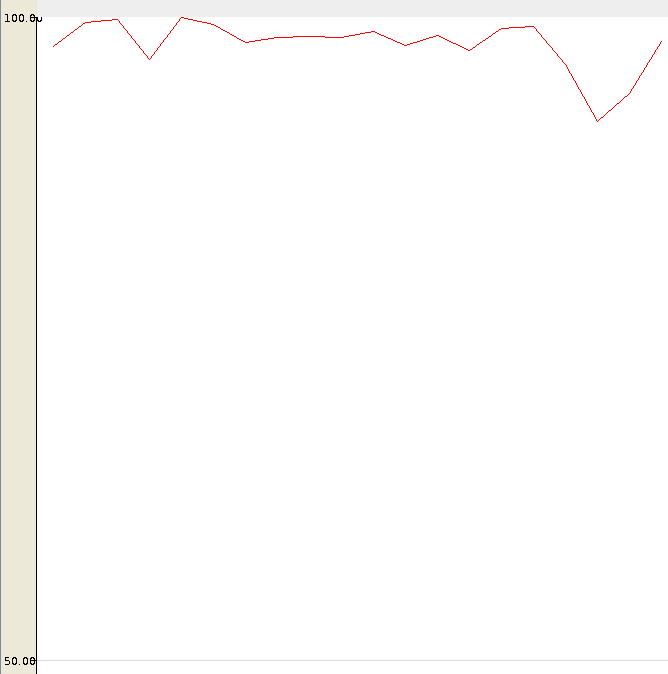
\includegraphics[width=0.5\linewidth]{2_5_1.png}
\end{figure}

\subsubsection{Ejercicio 2.}

\textbf{Repita el paso anterior cambiando el clasificador HoeffdingTree por un clasificador HoeffdingTree adaptativo.} \\

Para resolver este problema se ha usado la siguiente orden:

\begin{lstlisting}[language=bash]
EvaluatePrequential 
	-l (drift.SingleClassifierDrift -l trees.HoeffdingAdaptiveTree)
	-s (generators.RandomRBFGeneratorDrift 
		-r 1 
		-i 1 
		-a 7 
		-n 3
		-k 3 
		-s 0.001 
	) -i 2000000
-f 100000
\end{lstlisting}

El código es el mismo, sólo tenemos que cambiar el modelo que vamos a aprender en la línea dos. Las semillas se han cambiado tanto para la generación del modelo como para la generación de las instancias. Los resultados obtenidos son los siguientes:

\begin{table}[H]
	\centering
	\begin{tabular}{rcc}
		\textbf{Semilla} & \textbf{\% Acierto} & \textbf{Kappa} \\ \hline
		1 & 97.3 & 94.579 \\
		2 & 93.3 & 71.189 \\
		3 & 95.4 & 90.269 \\
		4 & 95.2 & 90.223 \\
		5 & 92.7 & 85.220
	\end{tabular}
\end{table}

La evolución de la curva de aciertos es la siguiente:

\begin{figure}[H]
	\centering
	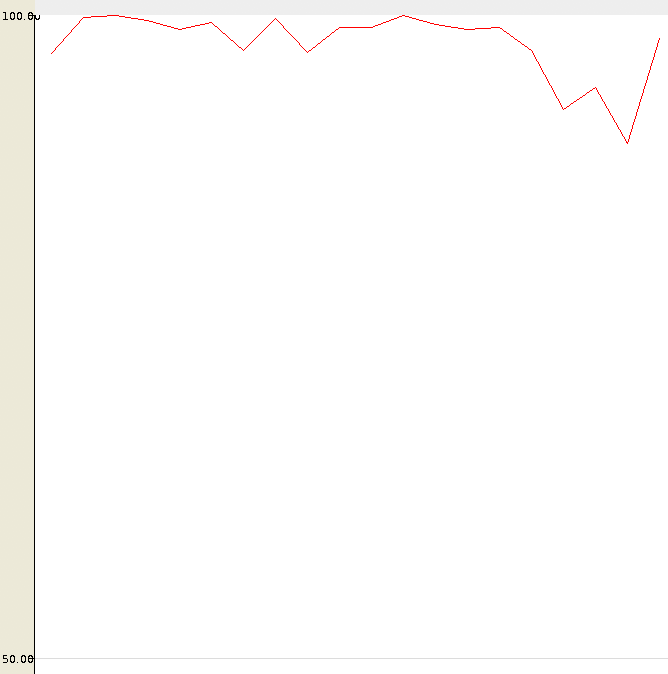
\includegraphics[width=0.5\linewidth]{2_5_2.png}
\end{figure}

Como parte extra, vamos a comparar ambos experimentos, tal y como hemos hecho en los apartados anteriores:

\begin{lstlisting}
shapiro.test(accuracy.standard)$p.value # 0.07903595
shapiro.test(kappa.standard)$p.value # 0.106312
shapiro.test(accuracy.adaptative)$p.value # 0.7089297
shapiro.test(kappa.adaptative)$p.value # 0.2067483

tseries::jarque.bera.test(accuracy.standard)$p.value # 0.6983299
tseries::jarque.bera.test(kappa.standard)$p.value # 0.6258841
tseries::jarque.bera.test(accuracy.adaptative)$p.value # 0.8432267
tseries::jarque.bera.test(kappa.adaptative)$p.value # 0.6330029
\end{lstlisting}

Cómo podemos ver, los datos son normales, así que podemos aplicar un test de \textit{Student}:

\begin{lstlisting}
t.test(accuracy.standard, accuracy.adaptative)$p.value # 0.7302075
t.test(kappa.standard, kappa.adaptative)$p.value # 0.8844594
\end{lstlisting}

Los test no si pasan, ya que el p-valor obtenido es mayor que 0.05, lo cual nos indica que no hay diferencia entre los algoritmos.

\subsubsection{Ejercicio 3.}

\textbf{Responda a la siguiente pregunta: ¿Qué diferencias se producen entre los métodos de los apartados 2.3, 2.4 y 2.5? Explique similitudes y diferencias entre las diferentes metodologías, y discuta los resultados obtenidos por cada una de ellas en el flujo de datos propuesto.} \\

Por lo general, dentro de cada experimento, el mejor resultado lo hemos obtenido usando la versión adaptativa del modelo \textit{HoeffdingTree}. Si comparamos los resultados obtenidos en los distintos experimentos podemos ver que, según avanzan los experimentos, obtenemos un modelo más estable. Veamos una tabla comparativa del acierto para la versión adaptativa del algoritmo: 

\begin{table}[H]
	\centering
	\begin{tabular}{rccc}
		\textbf{Semilla} & \textbf{2.3} & \textbf{2.4} & \textbf{2.5} \\ \hline
		1 & 96.249 & 96.6 & 97.3 \\
		2 & 92.647 & 95.3 & 93.3 \\
		3 & 96.309 & 98.0 & 95.4 \\
		4 & 95.983 & 96.3 & 95.2 \\
		5 & 90.996 & 91.9 & 92.7 \\ \hline
		\textbf{media} & 94.4368 & 95.62 & 94.78
	\end{tabular}
\end{table}

Aunque no haya mucha diferencia, podemos ver como, los modelos de los experimentos \textit{2.4} y \textit{2.5} son mejores. Esto se debe a que son experimentos donde se han introduzo técnicas para que el modelos se adapte mejor a los cambios de contexto, lo cual es la mayor diferencia de estos experimentos con el \textit{2.3}. La diferencia entre los experimentos \textit{2.4} y \textit{2.5} es el cómo se trabaja el cambio de contexto. En el primero (\textit{2.4}) se olvidan las instancias pasadas cuando se detecta el cambio de contexto mientras que en el segundo (\textit{2.5}) se reinicializa el modelo cuando se detecta el cambio de contexto.

\end{document}